\chapter{Pendulum Motion}

\section{Introduction}

In this lab we will apply the Euler and Verlet methods to the pendulum
problem.  We will compare the results of the Verlet problem to the
small angle approximation.

\section{Preparation}

Suppose you want to produce a plot of $f(t) = A \exp(-t/\lambda)$
versus $t$ from $t=0$ to $10$ and $A=\lambda=5$.  For a visually
smooth plot, you want about $N=100$ points, but we'll start with a
smaller number $N=11$ for easy debugging.  You create an array containing the 11
time values you want to plot:
\begin{python}
MAX = 10
N = 11
t = np.linspace(0,MAX,N)
print(t)
\end{python}
You calculate the $y = f(t)$ values like this:
\begin{python}
A    = 5
LAMB = 5
y = A*np.exp(-t/LAMB)  # !!!
print(y)
\end{python}
Make sure that you thoroughly understand the line marked ``!!!''.  That is
calculating one $y$ value for every $t$ value, and so $y$ is an array
with the same shape and size as $t$:
\begin{python}
print("t shape: ", np.shape(t), "y shape: ", np.shape(y))
print("t size:  ", np.size(t),  "y size: ", np.size(y))
\end{python}
With two arrays of the same shape, plotting them is a simple matter.  Here we use the red line format, and add some axes labels:
\begin{python}
plt.plot(t,y,"r-")
plt.xlabel("t (s)")
plt.ylabel("y")
\end{python}
If you look closely, you'll see kinks in the plot for $N=11$.  Increase to $N=100$ for a visually smooth plot.

\newpage

You are expected to do all of this on your own, from a prompt like this:\\

\plot Plot the function $f(t) = A \exp(-t/\lambda)$ from $t=0$ to 10, $A=5$ and $\lambda=5$ as a red line. \\

Now suppose instead that you already have a set of $y$-values in a \pyth{np.array} \pyth{yarr}, and you would like to plot $y$ vs $t$, knowing that these $y$ values were sampled starting at $t=0$ with a uniform step size of $\tau=0.2$ between each sample, i.e. at $t=0, 0.2, 0.4, \ldots$.  In this case, you would create a \pyth{np.array} containing your time values as:
\begin{python}
tau = 0.2
t = np.arange(yarr.size)*tau
\end{python} 
\vskip 0.25cm

\plot Starting from the $y$ values contained in:
\begin{python}
yarr = np.array([1,1,1,2,4,7,3,2,1,1,0,0])
\end{python}
which you know correspond to time values starting at $t=0$ with constant step size $\tau=0.5$.  Plot $y$ vs $t$ as blue circles and add axes labels.

\section{Pendulum Motion}

In lecture we showed a pendulum of length $L$ can be described by the angle $\theta$ with respect to vertical (rest position), the angular velocity:
\begin{displaymath}
\omega = \frac{d\theta}{dt}
\end{displaymath}
and the angular acceleration:
\begin{displaymath}
\alpha = \frac{d\omega}{dt} = \frac{d^2\theta}{dt^2} 
\end{displaymath}
In a constant gravitational field with acceleration $g$, the angular acceleration is:
\begin{displaymath}
\alpha = -\frac{g}{L} \, \sin \theta
\end{displaymath}
Which we can write as:
\begin{displaymath}
\alpha = - \omega_L^2 \, \sin \theta
\end{displaymath}
where
\begin{displaymath}
\omega_L = \sqrt{\frac{g}{L}}.
\end{displaymath}
This problem, which is quite simple to pose, has no analytic solution
in terms of elementary functions.  Instead, we will rely on numerical
techniques to solve it.\\

\section{Small Angle Approximation}

\begin{figure}[htbp]
\begin{center}
 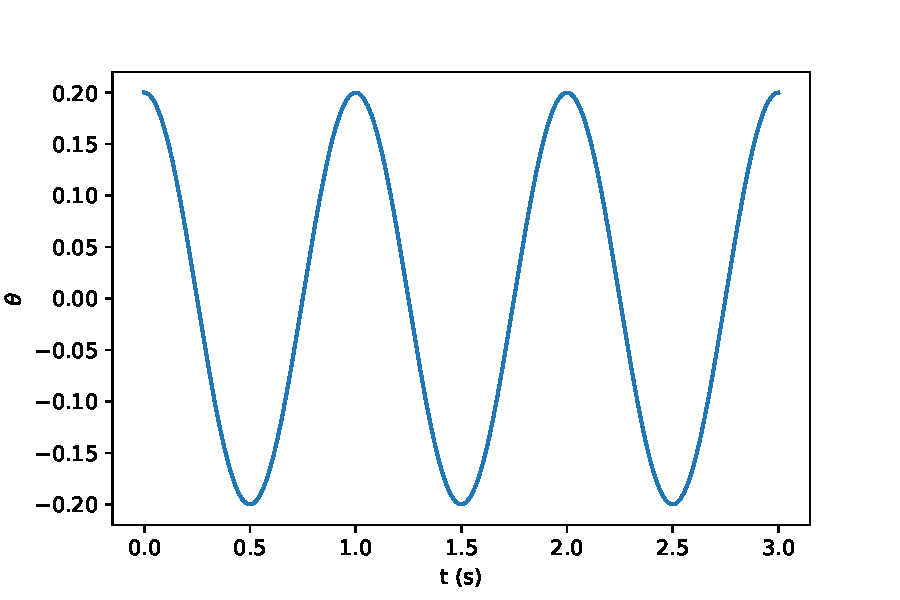
\includegraphics[height=0.33\textheight]{figs/pendulum/sho.pdf} 
\caption{The small angle approximation for pendulum motion with period $T_L=1~\rm s$}.
\label{fig:sho}
\end{center}
\end{figure}


Analytic solutions are the precious gems that we use to validate our
numerical techniques.  We'll start our analysis in a region where we
can solve the problem analytically.  For small displacements of the
pendulum, $\theta$ is small, and so:
\begin{displaymath}
\sin \theta \approx \theta
\end{displaymath}
and
\begin{displaymath}
\alpha = -\omega_L^2 \, \sin \theta \approx -\omega_L^2 \, \theta
\end{displaymath}
The differential equation which describes the motion is:
\begin{displaymath}
\frac{d^2\theta}{dt^2} = -\omega_L^2 \, \theta
\end{displaymath}
We showed in lecture that if the initial angular velocity is zero ($\omega_0 = 0$) and the initial theta position is $\theta_0$, then the solution is:
\begin{equation}
\label{eqn:sho}
\theta(t) = \theta_0 \cos(\omega_L \, t)
\end{equation}
as plotted in Fig.~\ref{fig:sho}.  The pendulum rocks back and forth
following a sine wave with period:
\begin{displaymath}
T_L = \frac{2 \pi}{ \omega_L} = 2 \pi \sqrt{\frac{L}{g}}
\end{displaymath}


\plot Calculate $\omega_L$ for a pendulum with $L=1~\rm m$ and $g=9.8~\rm m/s^2$.
What are the units of $\omega_L$?\\

\plot  Suppose you want to construct a pendulum such that for small
oscillations the period $T_L = 1~\rm s$.  What should be the value of
$\omega_L$?  What length $L$ should you use, assuming that $g=9.8~\rm
m/s$?\\

\newpage

\plot Reproduce the plot in Fig.~\ref{fig:sho}.  Set the
constants $T_L$, $\omega_L$, $\theta_0$, and $N$ as follows:
\begin{python}
TL = 1          # period in seconds 
wL = 2*np.pi/TL # small-angle angular frequency of pendulum 
A  = 0.2        # theta at t=0 (amplitude)
\end{python}
You must complete this problem {\bf without using an explicit for
  loop} and only {\bf six or less additional lines of code.}  (Debugging
print statements do not count toward this limit, use as many of those
as you like!)  To set the $y$ axis label to the fancy $\theta$ do:
\begin{python}
plt.ylabel("$\\theta$")
\end{python}.

\section{The Failure of the Euler Method}

The Euler equations for angle $\theta$ and angular velocity $\omega$ are:
\begin{eqnarray}
  \theta_{n+1} &=& \theta_n + \tau \, \omega \\
  \omega_{n+1} &=& \omega_n + \tau \, \alpha 
\end{eqnarray}
where $\alpha$ is the angular acceleration and $\tau$ is the time step.\\

\plot Implement a function
\begin{python}
def euler(tau, theta, omega, alpha):
   # your code here
   return theta, omega
\end{python}
which implements one iteration of the Euler method.
Test your \pyth{euler} function with these test values:
\begin{python}
print(np.around(euler(-0.01, -0.28, -0.30, -0.06),3))
print(np.around(euler( 0.94,  0.32, -0.85, -0.86),3))
print(np.around(euler( 0.92, -0.16,  0.38, -0.32),3))
print(np.around(euler( 0.31,  0.12, -0.91, -0.76),3))
print(np.around(euler(-0.14,  0.96,  0.66, -0.73),3))
\end{python}
which should produce the following output:
\begin{verbatim}
[-0.277 -0.299]
[-0.479 -1.658]
[0.19  0.086]
[-0.162 -1.146]
[0.868 0.762]
\end{verbatim}
You'll use this now thoroughly tested function more below.  Don't change it!\\

\plot  Apply the Euler method to the problem of small oscillations of a pendulum with $T_L=1~\rm s$ as in Fig.~\ref{fig:sho}.  First, set the parameters of your code just as before:
\begin{python}
TL = 1          # period in seconds 
wL = 2*np.pi/TL # small-angle angular frequency of pendulum 
A  = 0.2        # theta at t=0 (amplitude)
\end{python}
Then implement the Euler method as follows:
\begin{algorithm}
  $\theta$ := A
  $\omega$ := 0
  $\tau$ := 0.0003
  Create an empty array tjth which will contain $\theta$ positions of the trajectory
  Append $\theta$ to the array tjth.
  Repeat $N$ times:
     Calculate $\alpha = \omega_L^2 \theta$
     Update $\theta$ and $\omega$ for acceleration $\alpha$ and time step $\tau$ by calling euler().
     Append $\theta$ to the array tjth.
  Create an array t containting $N+1$ appropriately spaced time values.
  Plot tjth versus t
\end{algorithm} 
As always, first debug your code using a small value for $N$.  Then,
you should reproduce something that closely resembles Fig.~\ref{fig:sho} with
$N=10000$. \\

\plot Repeat the exercise above (you can use cut and paste) with $\tau=0.01$ and $N=1000$.  Yikes!  Is energy conserved?\\

\section{The Verlet Method}

The Verlet Equation for this problem is:
\begin{eqnarray}
  \theta_{n+1} &=& 2 \theta_n - \theta_{n-1} + \tau^2 \, \alpha
\end{eqnarray}
Notice that with the Verlet method, we will not need to calculate angular
velocity $\omega$ in order to get the $\theta$ trajectory.\\

\plot Implement a function
\begin{python}
def verlet(tau, theta, oldth, alpha):
   # your code here
   return theta
\end{python}
which returns $\theta_{n+1}$ from $\theta_n=$theta and
$\theta_{n-1}=$oldth using the verlet method.
Test your \pyth{verlet} function with these test values:
\begin{python}
print(np.around(verlet(-0.01, -0.28, -0.30, -0.06),3))
print(np.around(verlet( 0.94,  0.32, -0.85, -0.86),3))
print(np.around(verlet( 0.92, -0.16,  0.38, -0.32),3))
print(np.around(verlet( 0.31,  0.12, -0.91, -0.76),3))
print(np.around(verlet(-0.14,  0.96,  0.66, -0.73),3))
\end{python}
which should produce the following output:
\begin{verbatim}
-0.26
0.73
-0.971
1.077
1.246
\end{verbatim}
You'll use this now thoroughly tested function more below.  Don't change it!\\

\plot  In a previous exercise you showed that the Euler method, when applied to the problem of small oscillations of a pendulum with $T_L=1~\rm s$ for $\tau=0.01$ and $N=1000$, is unstable.  Instead, apply the Verlet method.  You can reuse (by copying and pasting) much of your code from that previous exercise with a few changes:
\begin{itemize}
 \item You will call your \pyth{verlet} function instead of \pyth{euler}.
 \item You no longer need to keep track of $\omega$ (\pyth{omega})
 \item You will now have to keep track of two $\theta$ values at all times.  At each updat:
\begin{displaymath}
   (\theta_n, \theta_{n-1}) \rightarrow  (\theta_{n+1}, \theta_{n})
\end{displaymath}
 \item You can start things off with \pyth{oldth = theta = A}
\end{itemize}
With this method, you should produce many oscillations with no sign of instability.\\

\plot So far, we have been using the small angle approximation.  Modify your code to use the exact formula for the angular acceleration $\alpha = \omega_L^2 \, \sin \theta$ and set the initial position to $A=2$.  This is a trivial change to your numerical simulation, but it  makes an analytic solution impossible!\\

\plot (Optional Challenge) Run you Verlet analysis for $N=1000$ steps
for $A=3$ and set $\tau$ appropriately so that you see a bit more than
one period of motion.  Plot the trajectory as a black line and read
off the period $T$.  Superimpose a plot of a cosine with amplitude $A$
and period $T$.\\

\plot (Optional Challenge) We've been starting things off with
approximately zero angular velocity by setting
\pyth{oldth = theta = A}.
You can add velocity to the initial state with:
\begin{python}
  V = 1
  theta = A
  oldth = A - tau*V
\end{python}
Give the pendulum enough of a whack that it reaches all the way to top
and keeps going.  When plotting this trajectory, you can use \pyth{np.mod} to
keep the theta values in the range from -$\pi$ to $\pi$ if you want.\\

\plot (Optional Challenge) Fix the Euler method for this pendulum
problem by forcing energy to be conserved at each step.  Compare your
results to the Verlet method.\\















